\documentclass[10pt,letterpaper,notitlepage]{article}
\usepackage[utf8]{inputenc}
\usepackage[T1]{fontenc}
\usepackage{amsmath}
\usepackage{amsfonts}
\usepackage{amssymb}
\usepackage{graphicx}
\usepackage{hyperref}
\usepackage{derivative}
\usepackage{cleveref}
\usepackage[backend=biber]{biblatex}
% \addbibresource{hw4.bib}
\author{Mike Sutherland}
\title{MAE 195 HW 4 Assignment}
\begin{document}
    \maketitle
    % \printbibliography
    \section{Problem 1}
    We consider a 2nd order ordinary differential equation of the form
    \begin{equation}
        \begin{aligned}
            \ddot{x} + \alpha \dot{x} + \omega_0^2 x &= 0 \\
            x(0) &= x_0 \\
            \dot{x}(0) &= \dot{x}_0
        \end{aligned}
        \label{eq:problem1}
    \end{equation}
    We can re-write this system in state-space form:
    \begin{equation}
        \begin{bmatrix}
            \dot{x} \\
            \ddot{x}
        \end{bmatrix}
        =
        \begin{bmatrix}
            0 & 1 \\
            -\omega_0^2 & -\alpha
        \end{bmatrix}
        \begin{bmatrix}
            x \\
            \dot{x}
        \end{bmatrix}
    \end{equation}
    Let's attach some names to these terms. We will rename our state $\begin{bmatrix}
        x \\
        \dot{x}
    \end{bmatrix}$ simply to $x$. Then, our equation takes the form:
    \begin{equation}
        \begin{aligned}
            \dot{x} &= A x \\
            \frac{dx}{dt} &= A x(t)
        \end{aligned}
    \end{equation}
    In this form, the properties of $A$ will determine the behavior of the system and its numerical attributes. We begin with the eigenvalues of A:
    \begin{equation}
        \begin{aligned}
            \lambda_1 &= -\frac{\alpha}{2} - \frac{\sqrt{\alpha^2 - 4 \omega_0^2}}{2} \\
            \lambda_2 &= -\frac{\alpha}{2} + \frac{\sqrt{\alpha^2 - 4 \omega_0^2}}{2}
        \end{aligned}
    \end{equation}
    Depending on the sign and size of $\alpha$ and $\omega_0$, the eigenvalues will either be real or complex. Let us assume that both $\alpha$ and $\omega_0$ are positive, as they would be in a physical spring-mass system. In that case, if $\alpha^2 \leq 4 \omega_0^2$, then we have complex eigenvalues. (physically, these will produce some oscillations in the spring).
    The spectral condition number is:
    \begin{equation}
        \begin{aligned}
            \kappa &= \frac{|\text{Re}(\lambda_1)|}{|\text{Re}(\lambda_2)|} \\
            \kappa &= \frac{| \text{Re}(\alpha + \sqrt{\alpha^2 - 4 \omega_0^2})|}{|\text{Re}(\alpha - \sqrt{\alpha^2 - 4 \omega_0^2})|}
        \end{aligned}
    \end{equation}
    So, we have 3 cases for this simple system: two real eigenvalues (overdamped), one repeated real eigenvalue (underdamped), and one complex eigenvalue (underdamped). We will analyze numerical solutions to two underdamped cases in \cref{sec:problem2,sec:problem3,sec:problem5}.
    \section{Problem 2}
    \label{sec:problem2}
    The analytic solution of \cref{eq:problem1}, for the cases presented in \cref{sec:problem3}, is:
    \begin{equation}
        x(t) = e^{\text{Re}(\lambda_1) t} (c_1 \cos(\text{Im}(\lambda_1) t) + c_2 \sin(\text{Im}(\lambda_1) t))
    \end{equation}
    The solution has the form of a sinusoid whose frequency is set by the imaginary component of $\lambda_1$ and whose amplitude is set by the decaying exponential envelope characterized by the real component of $\lambda_1$. Because the complex eigenvalues for this $2\times 2$ system arrive in a pair, it does not matter whether we use the first or second; the real component is identical and the two imaginary components are symmetrical.
    \section{Problem 3, 4}
    \label{sec:problem3}
    For problem 3, we have two cases. The first case is a non-stiff case and is analyzed in \cref{fig:problem31} and \cref{fig:problem31err}. We compare this case with the second case, which is stiff and is analyzed in \cref{fig:problem32} and \cref{fig:problem32err}. The spectral condition number, $\kappa$, is shown at the top of each plot.
    \begin{figure}
        \centering
        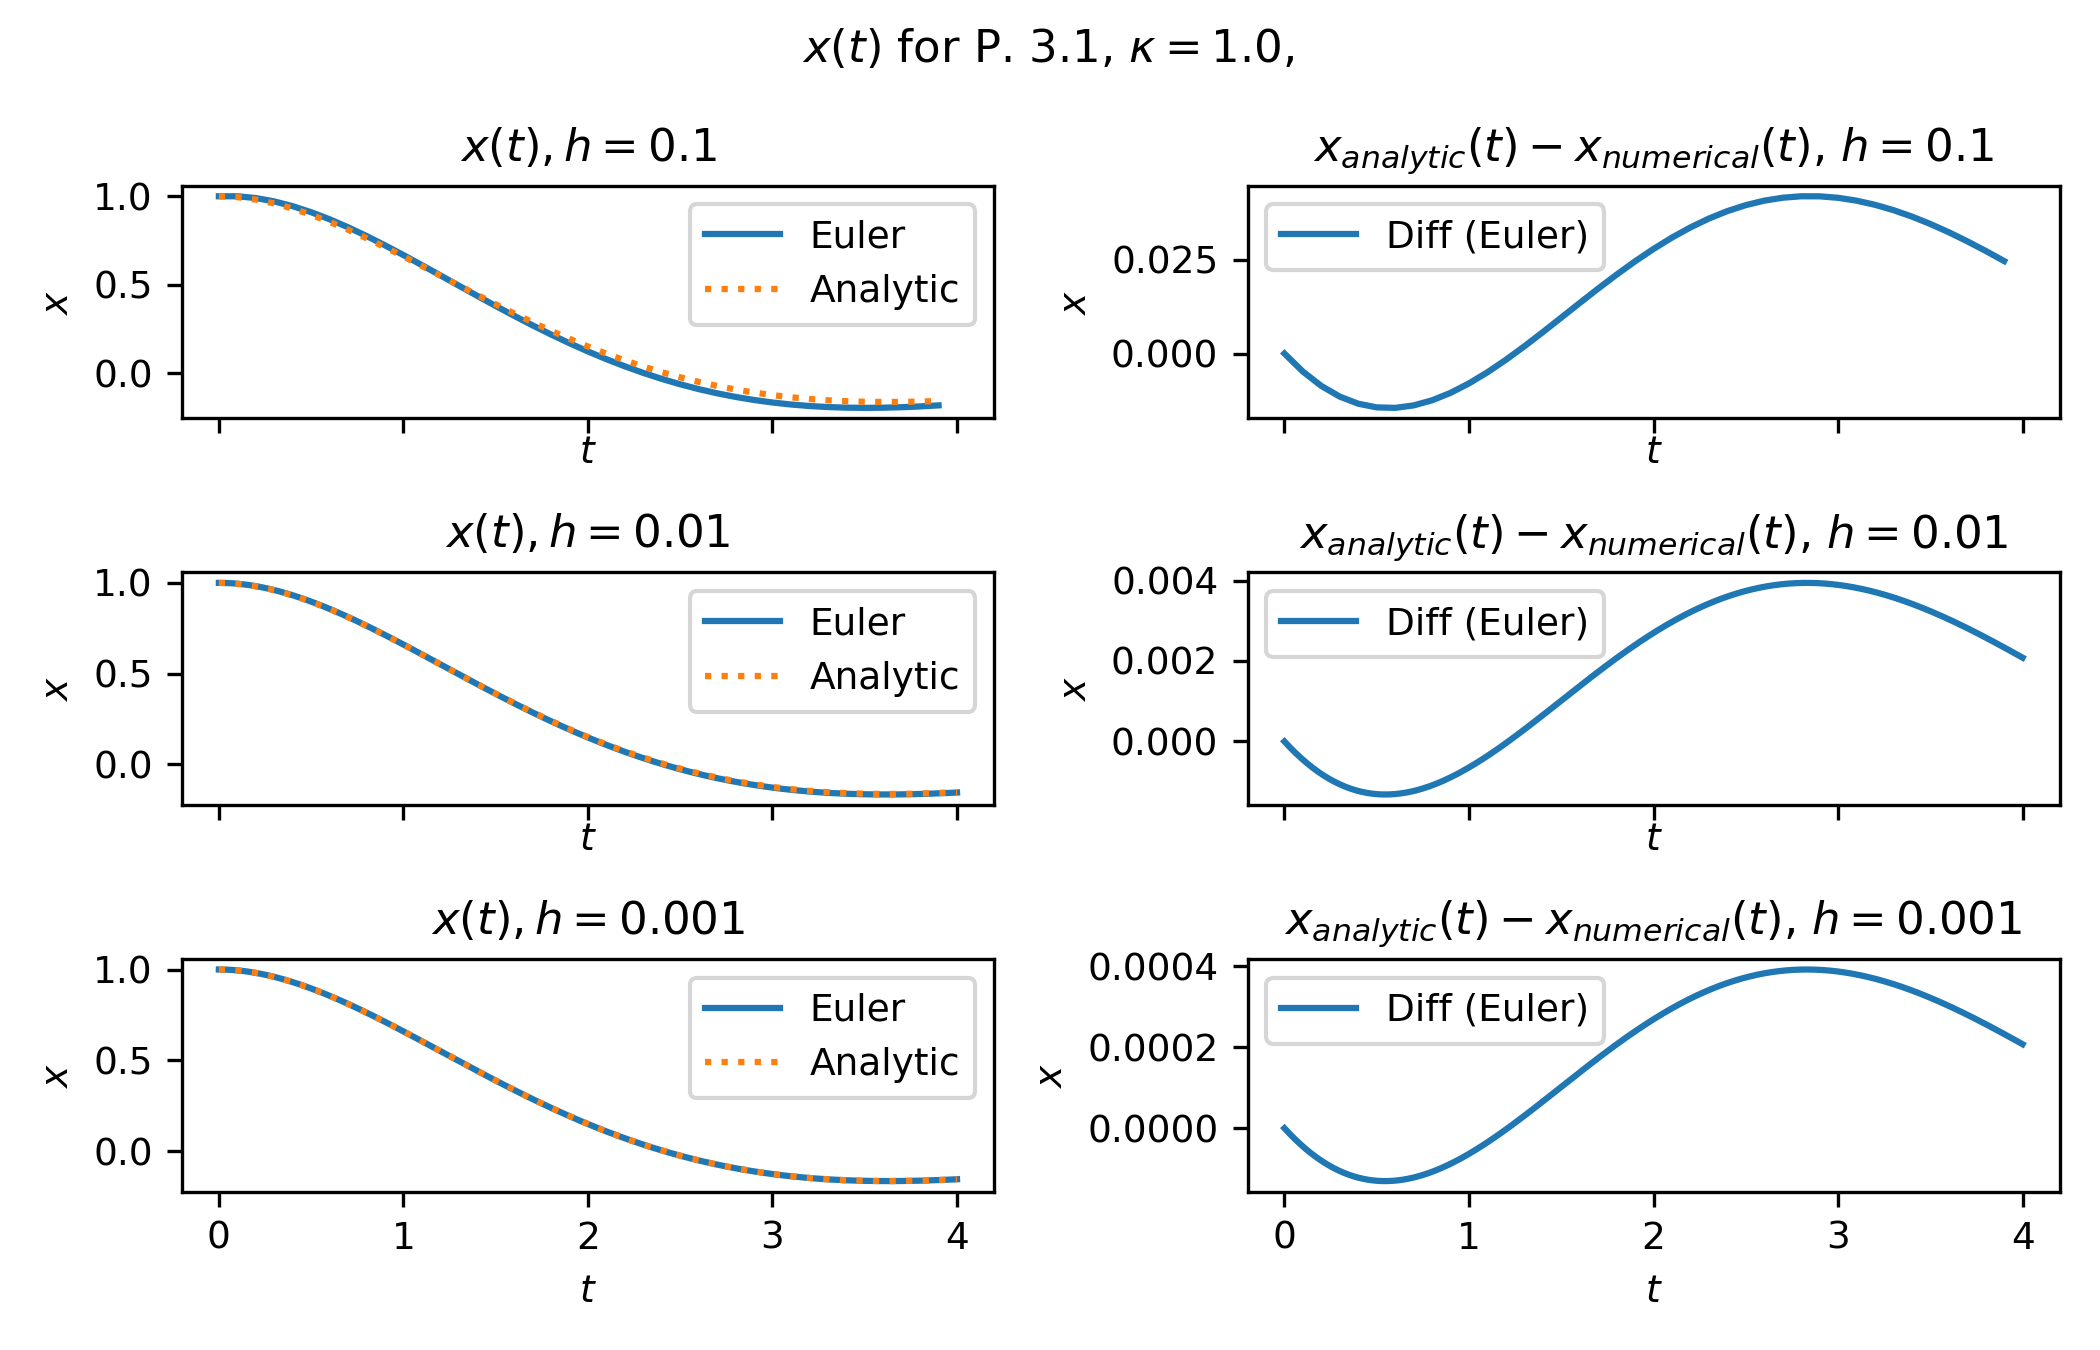
\includegraphics[width=0.9\textwidth]{../figures/p31.png}
        \caption{Problem 3, Case 1. This figure shows the analytic solution compared with the numerical solution for four different step sizes. In the left column, we see the solution $x(t)$ across the interval for both the analytic and numerically calculated solutions. In the right column, we see the difference between the numerical solution and the analytic solution ($x(t)_{\text{numeric}} - x(t)_{\text{analytic}}$). Note the change in scale in the y-axes.}
        \label{fig:problem31}
    \end{figure}
    \begin{figure}[h]
        \centering
        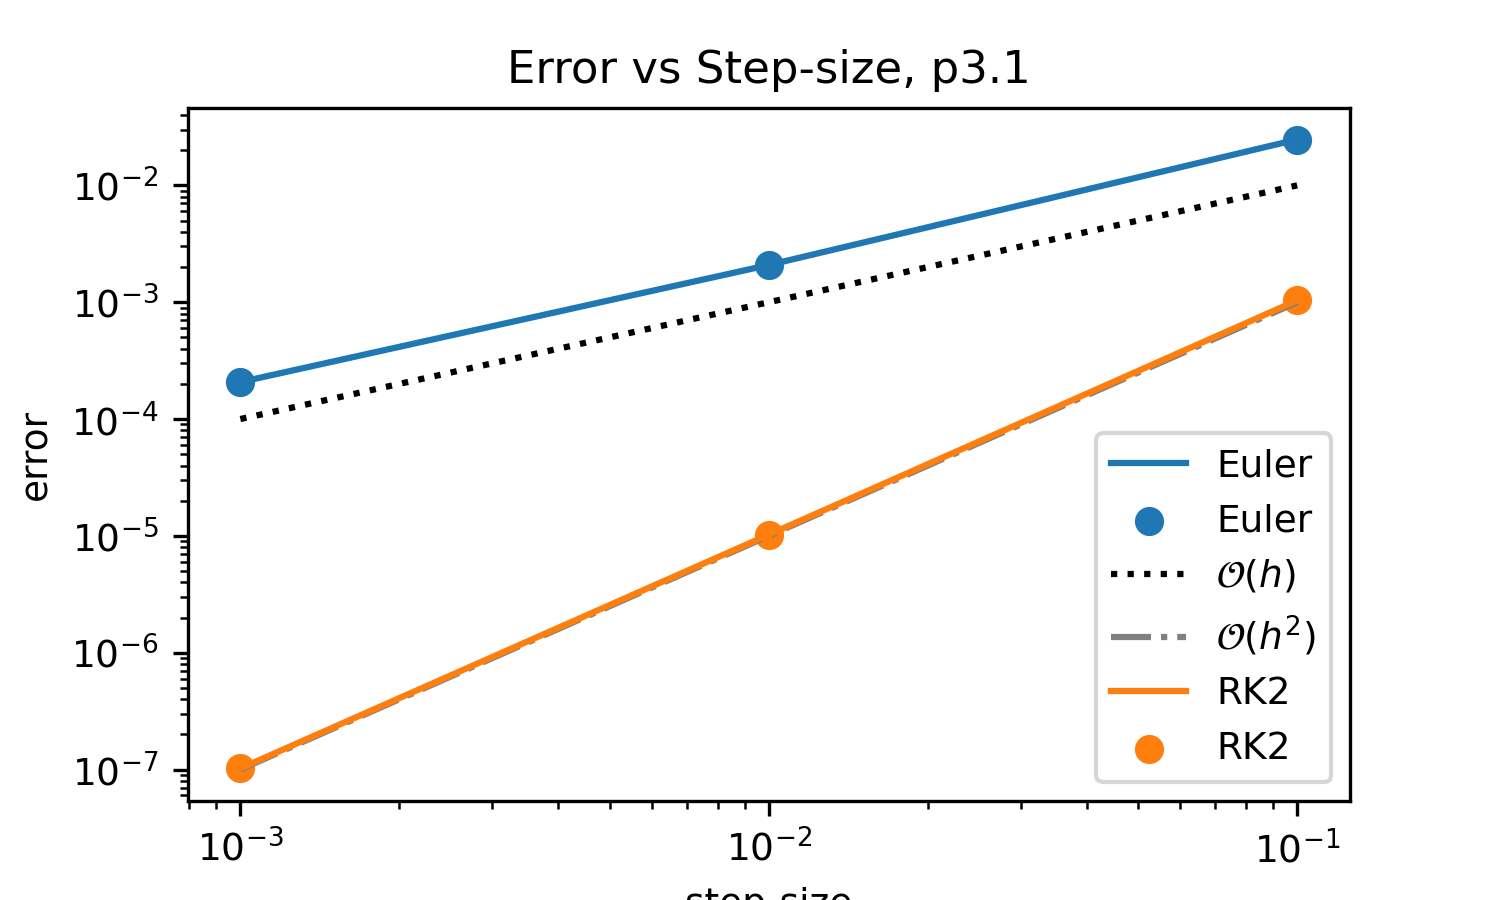
\includegraphics[width=0.9\textwidth]{../figures/p31err.png}
        \caption{Problem 3.1 and 4.1 error analysis. The error is measured at $t_{final}$, and plotted on log-log scale. We can see that the Euler method has identical slope to first order ($\mathcal{O}(n)$) error. Additionally, the error of a 2nd-order Runge-Kutta method is shown; we can see that it has identical slope to second order ($\mathcal{O}(n^2)$)error.}
        \label{fig:problem31err}
    \end{figure}
    \begin{figure}[h]
        \centering
        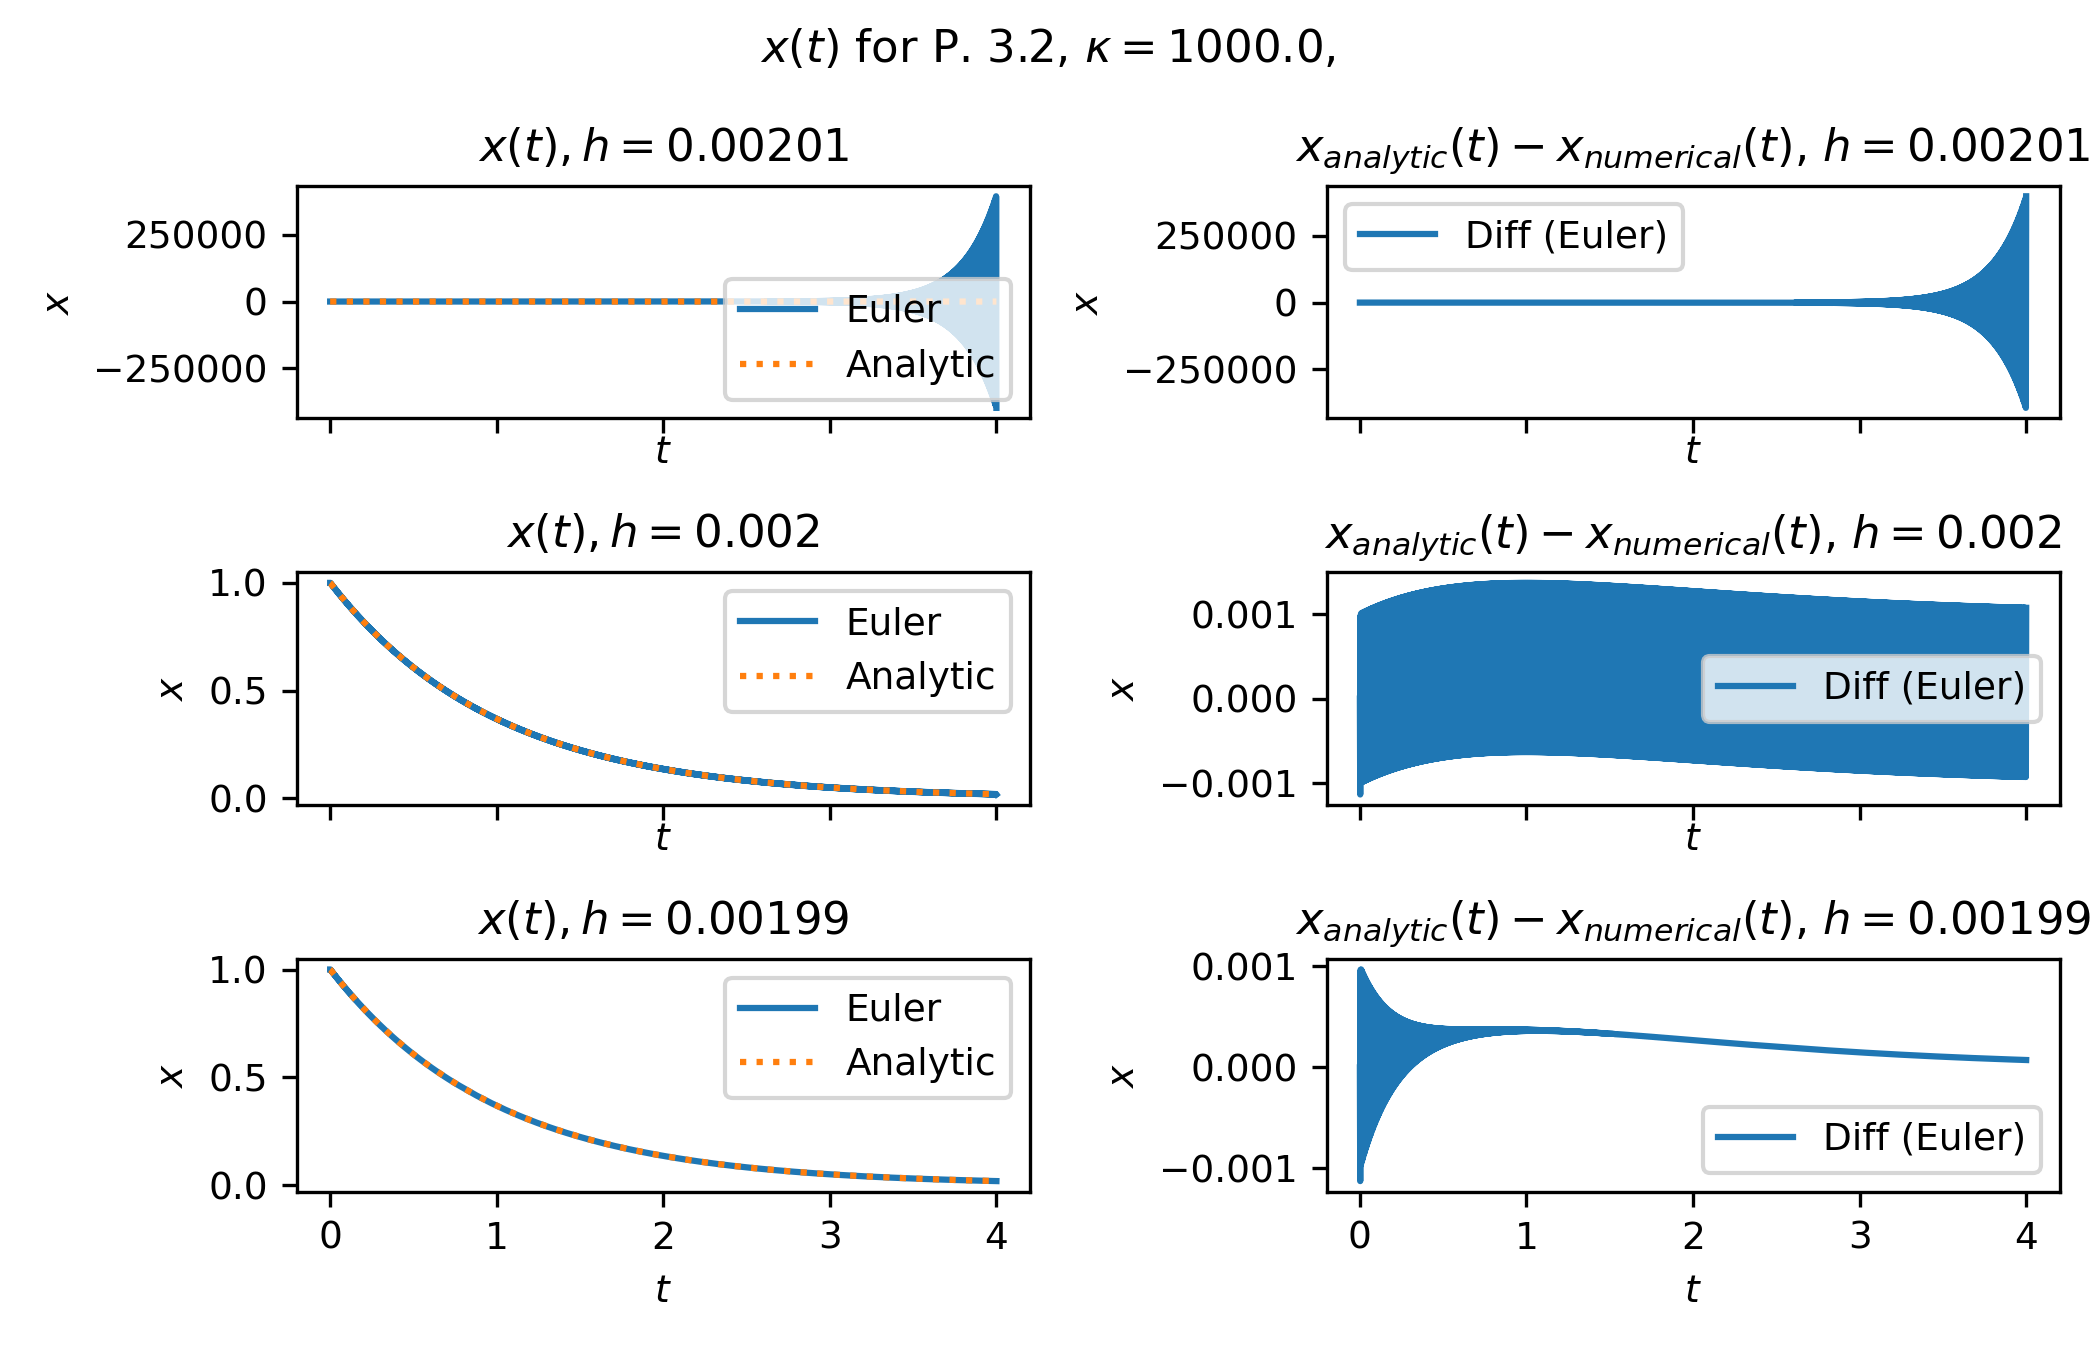
\includegraphics[width=0.9\textwidth]{../figures/p32.png}
        \caption{Problem 3.2. This plot shows a stiff problem (note the condition number). Again, the analytic and numerical solutions are shown in the left column, while the difference between them is shown in the right column. The step size of $h=0.002$ is exactly the "critical" step size; any higher, and the numerical solution fails to produce meaningful results. There are too many individual steps for their oscillations to be visible in the plot, but we can see the envelope of these oscillations in the right-hand column: when the step size $h\geq 0.002$, the numerical solution has greater error as the problem is solved forward; when the step size $h\leq 0.002$, the numerical solution has less error as the problem is solved forward.}
        \label{fig:problem32}
    \end{figure}
    \begin{figure}[h]
        \centering
        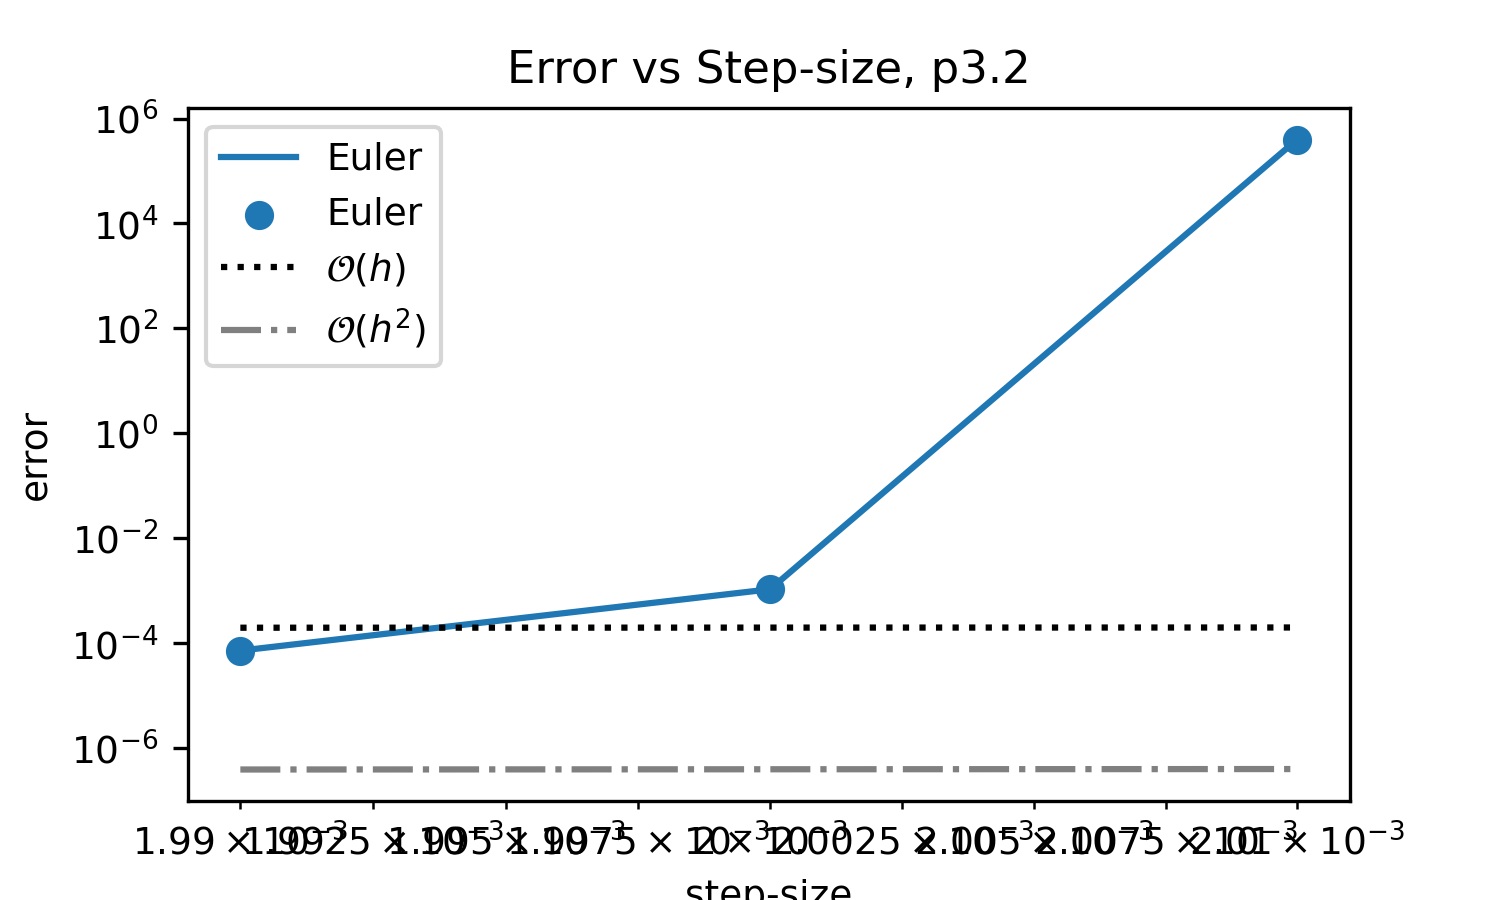
\includegraphics[width=0.9\textwidth]{../figures/p32err.png}
        \caption{The error for \cref{fig:problem32}. We can see that when the step size increases past the critical point of $h=0.002$, the error becomes unbounded. Otherwise, the error is $\mathcal{O}(n)$.}
        \label{fig:problem32err}
    \end{figure}
    \begin{figure}[h]
        \centering
        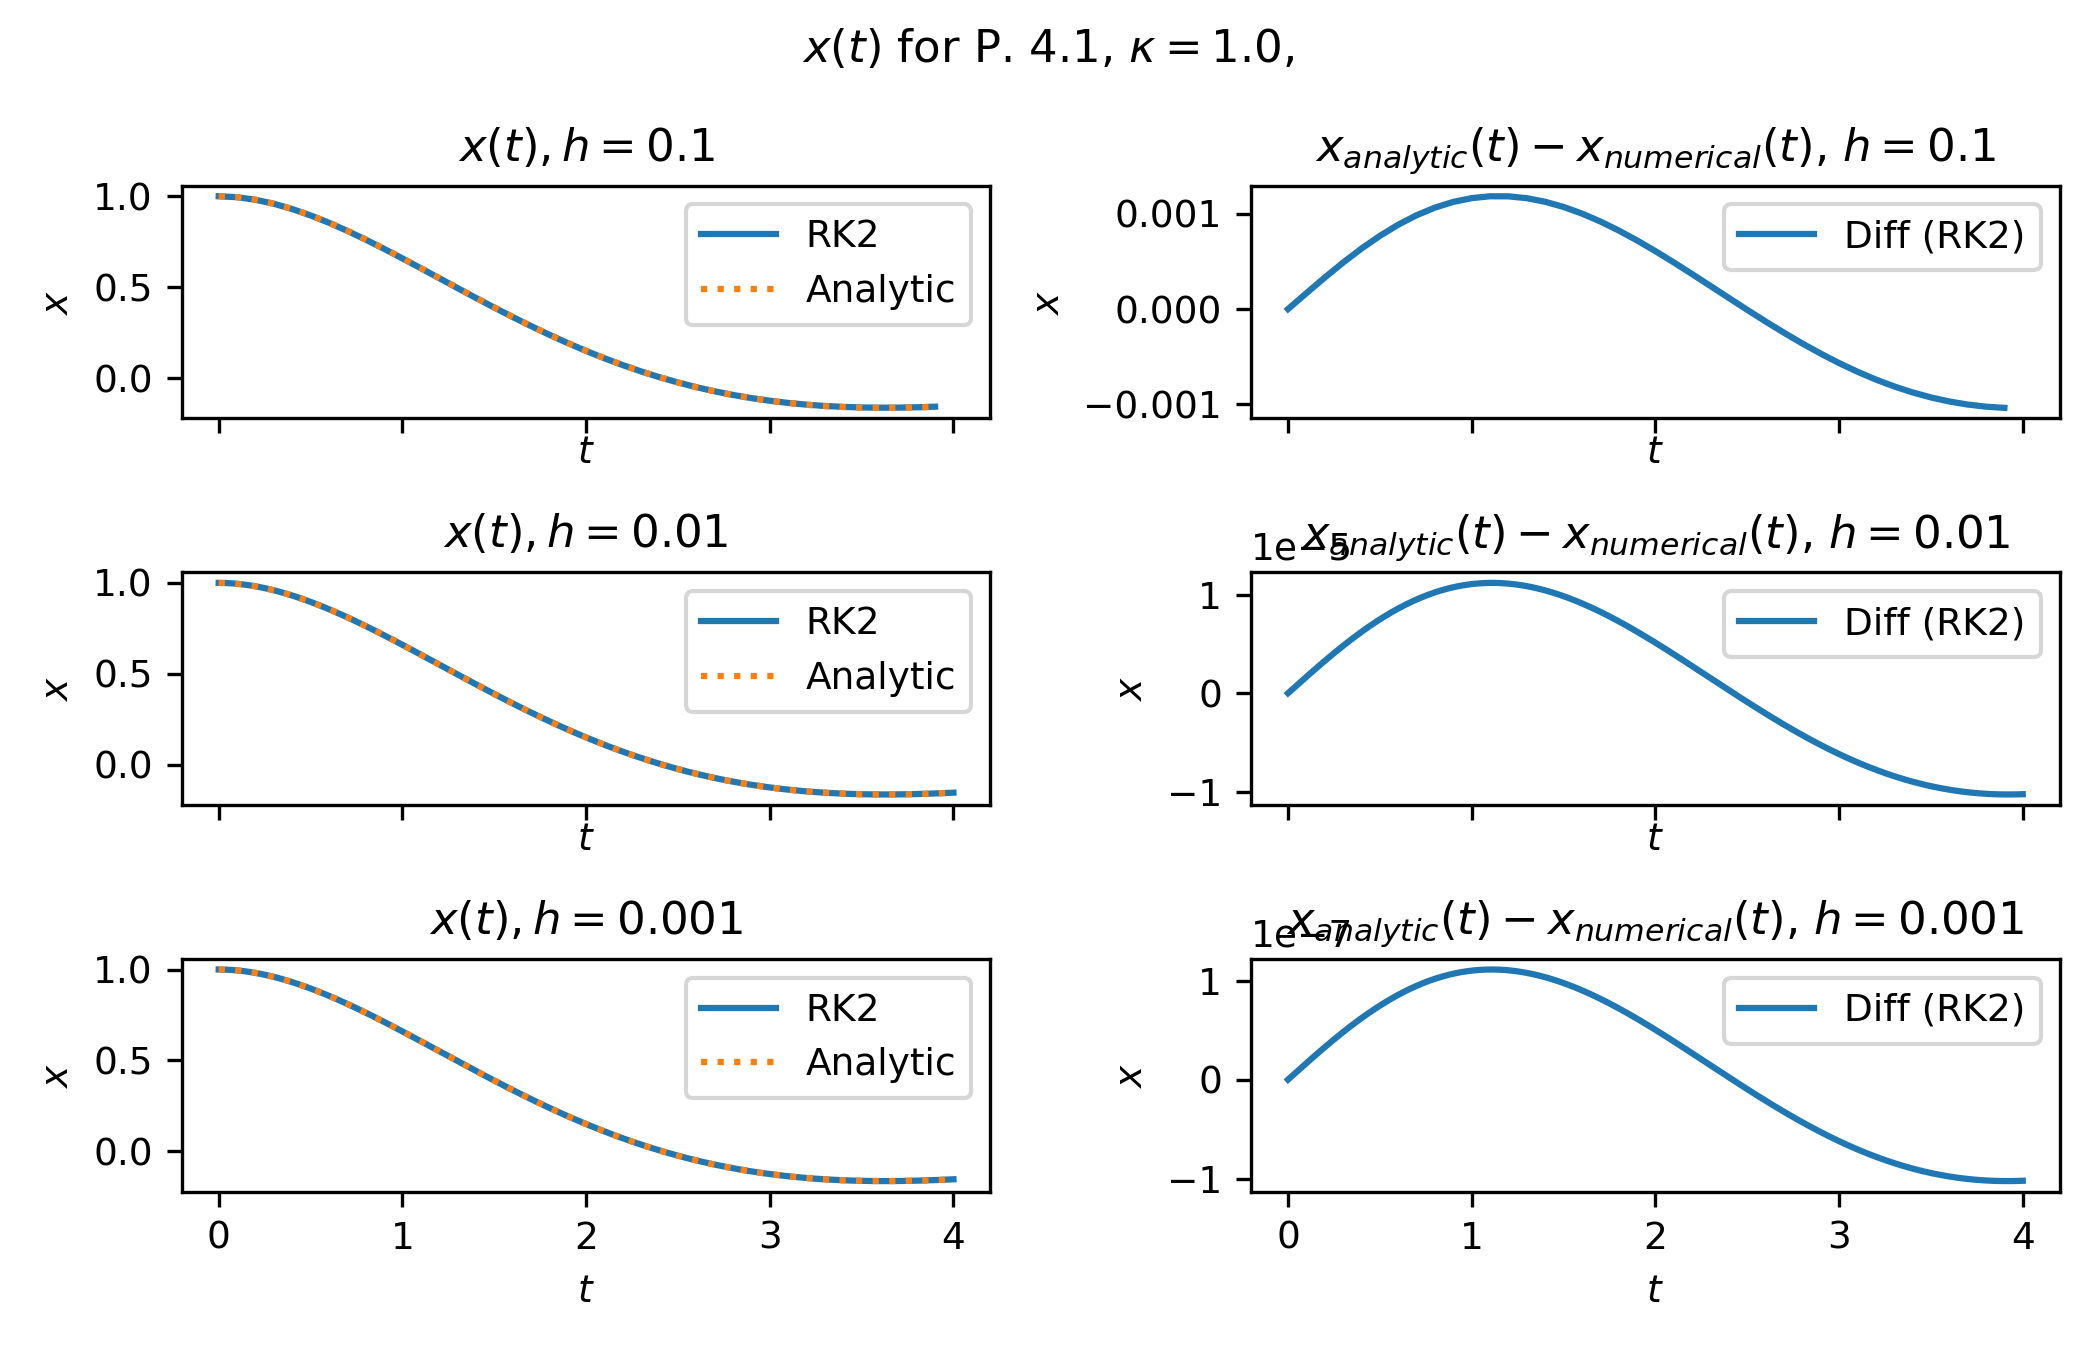
\includegraphics[width=0.9\textwidth]{../figures/p41.png}
        \caption{Problem 4, Case 1: 2nd order Runge-Kutta solver. We see that the error is smaller and decreases more rapidly for the Runge-Kutta solver. (See \cref{fig:problem31err} for error analysis.)}
    \end{figure}
 
    \section{Problem 5}
    \label{sec:problem5}
    Results for the same equation using an Adams Moulton solver. We can see that even with large step sizes, the solution remains stable (\cref{fig:problem51,fig:problem51err}), even for stiff problems (\cref{fig:problem52,fig:problem52err}). The tradeoff between implicit and explicit solvers is discussed in \cref{fig:problem52err}.
    \begin{figure}[h]
        \centering
        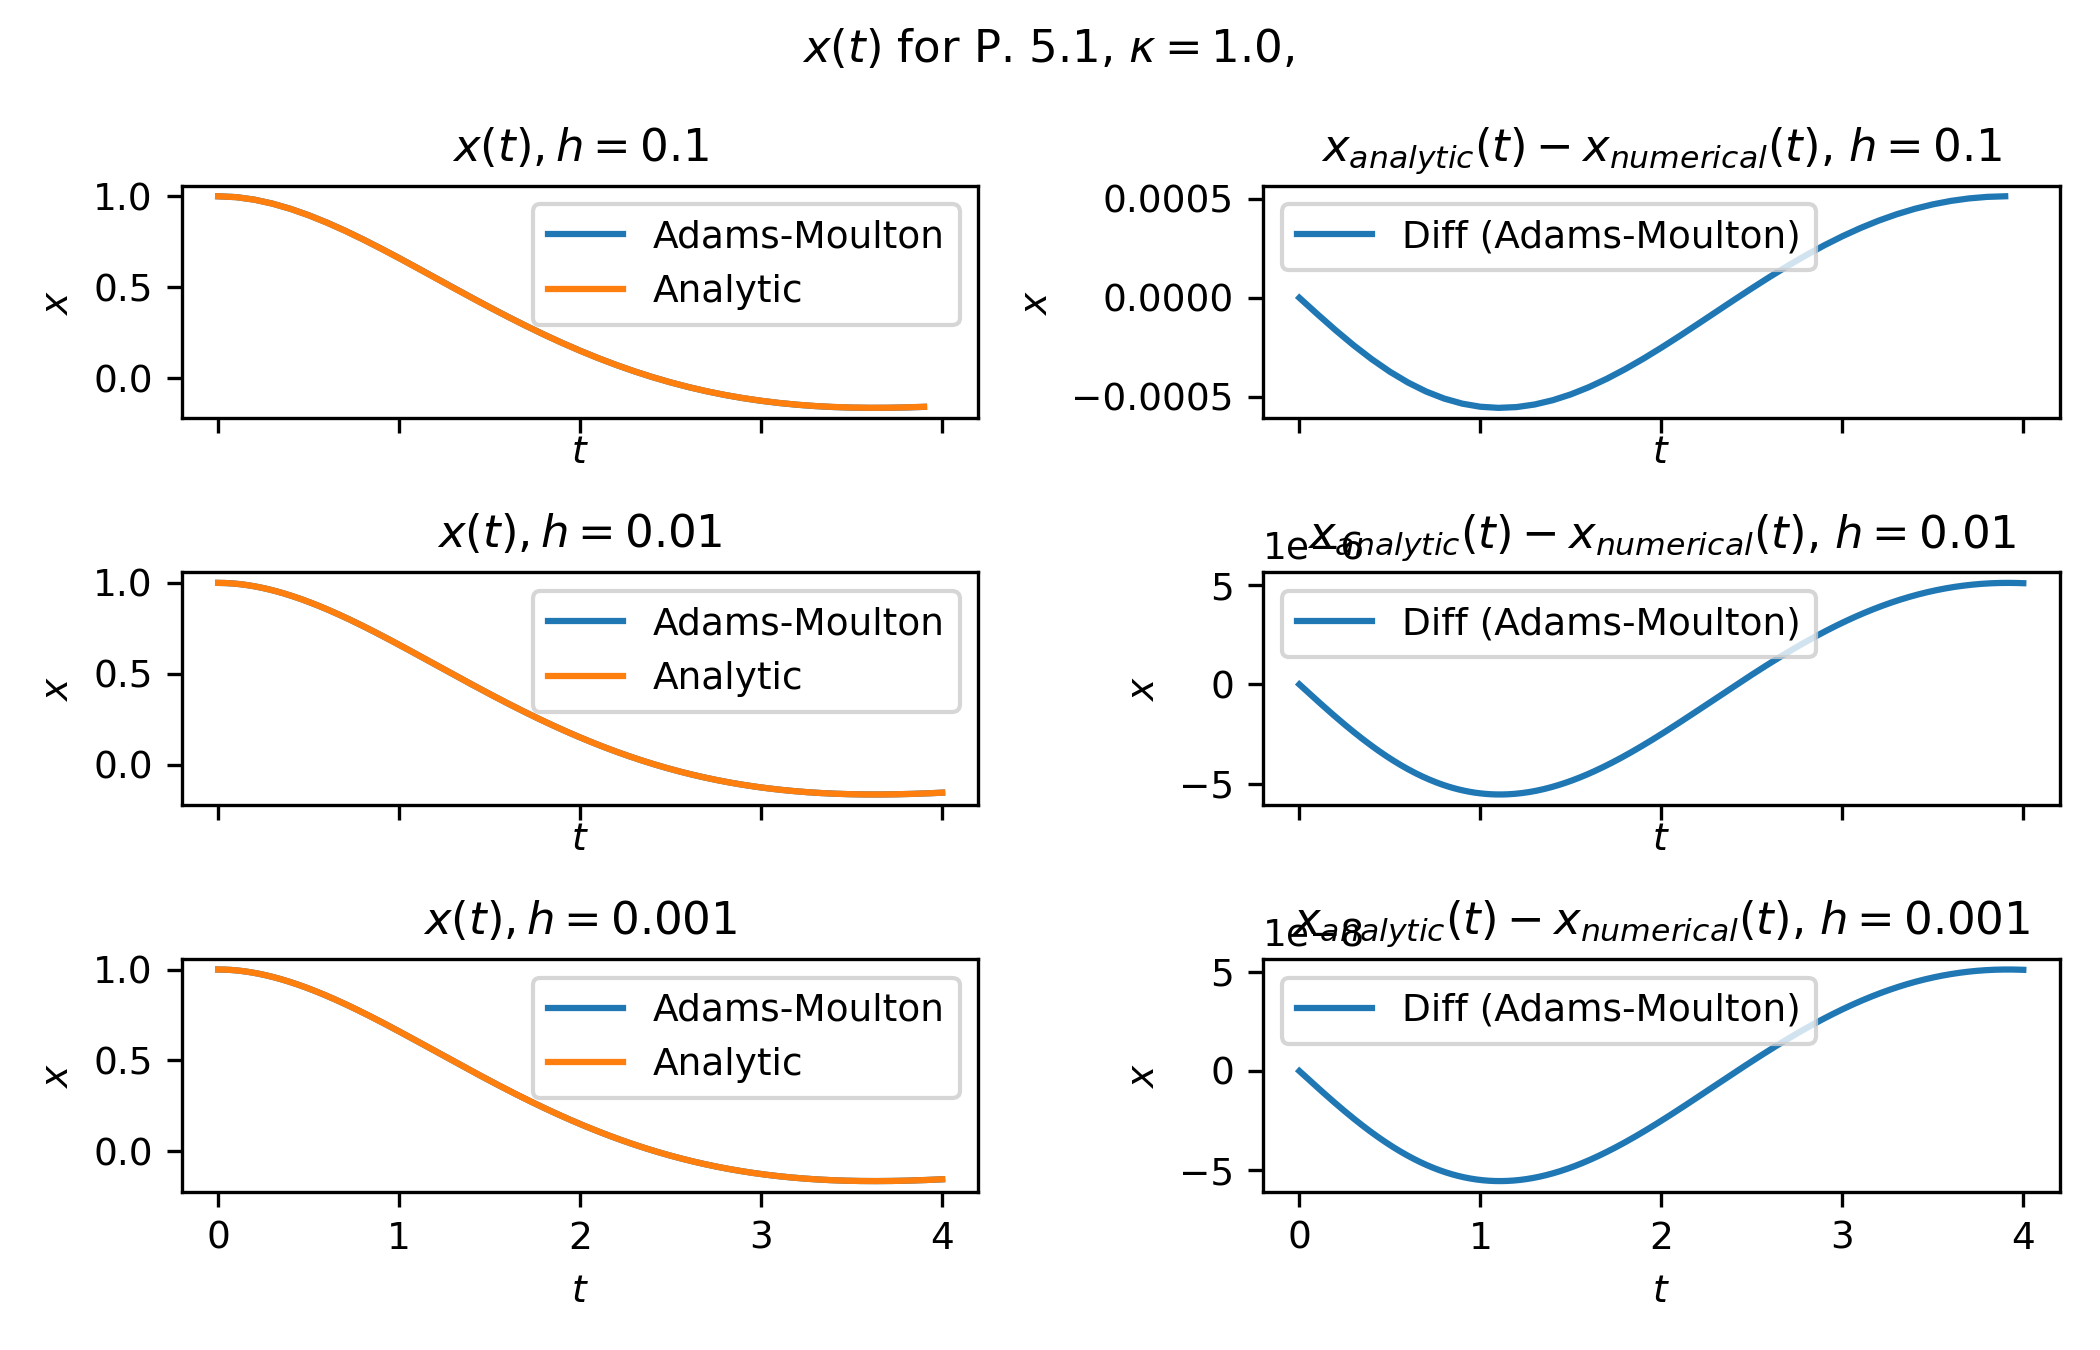
\includegraphics[width=0.9\textwidth]{../figures/p51.png}
        \caption{Problem 5.1. This plot shows the solution for the same problem using an Adams Moulton solver. The solution is stable for all step sizes.}
        \label{fig:problem51}
    \end{figure}
    \begin{figure}[h]
        \centering
        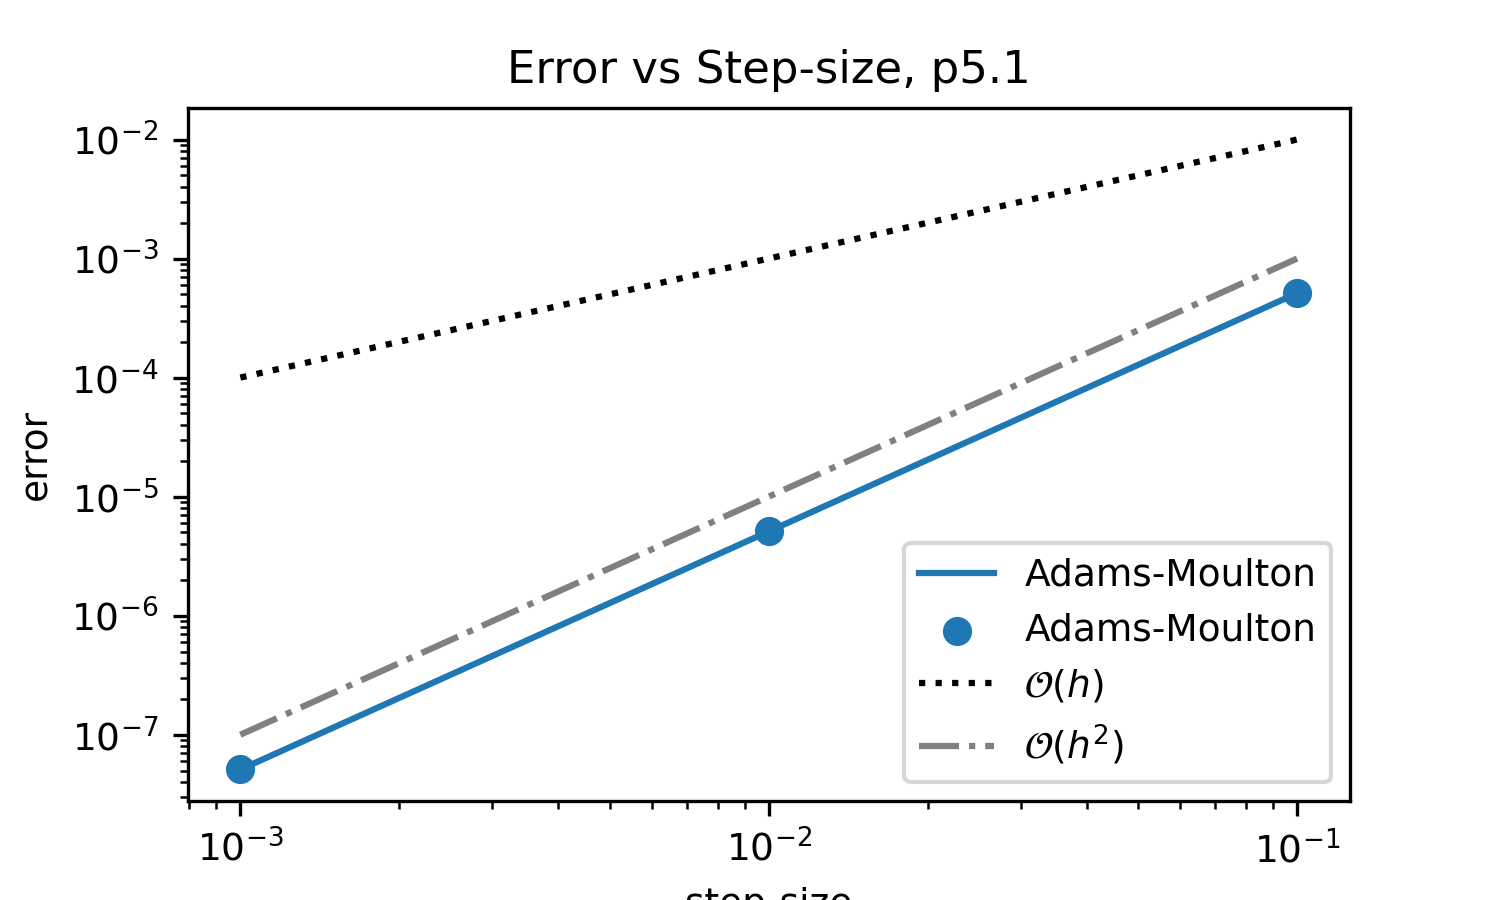
\includegraphics[width=0.9\textwidth]{../figures/p51err.png}
        \caption{Problem 5.1 error analysis. This plot shows an error analysis for the Adams-Moulton solver. We see that it is 2nd order accurate for Case 1.}
        \label{fig:problem51err}
    \end{figure}
    \begin{figure}[h]
        \centering
        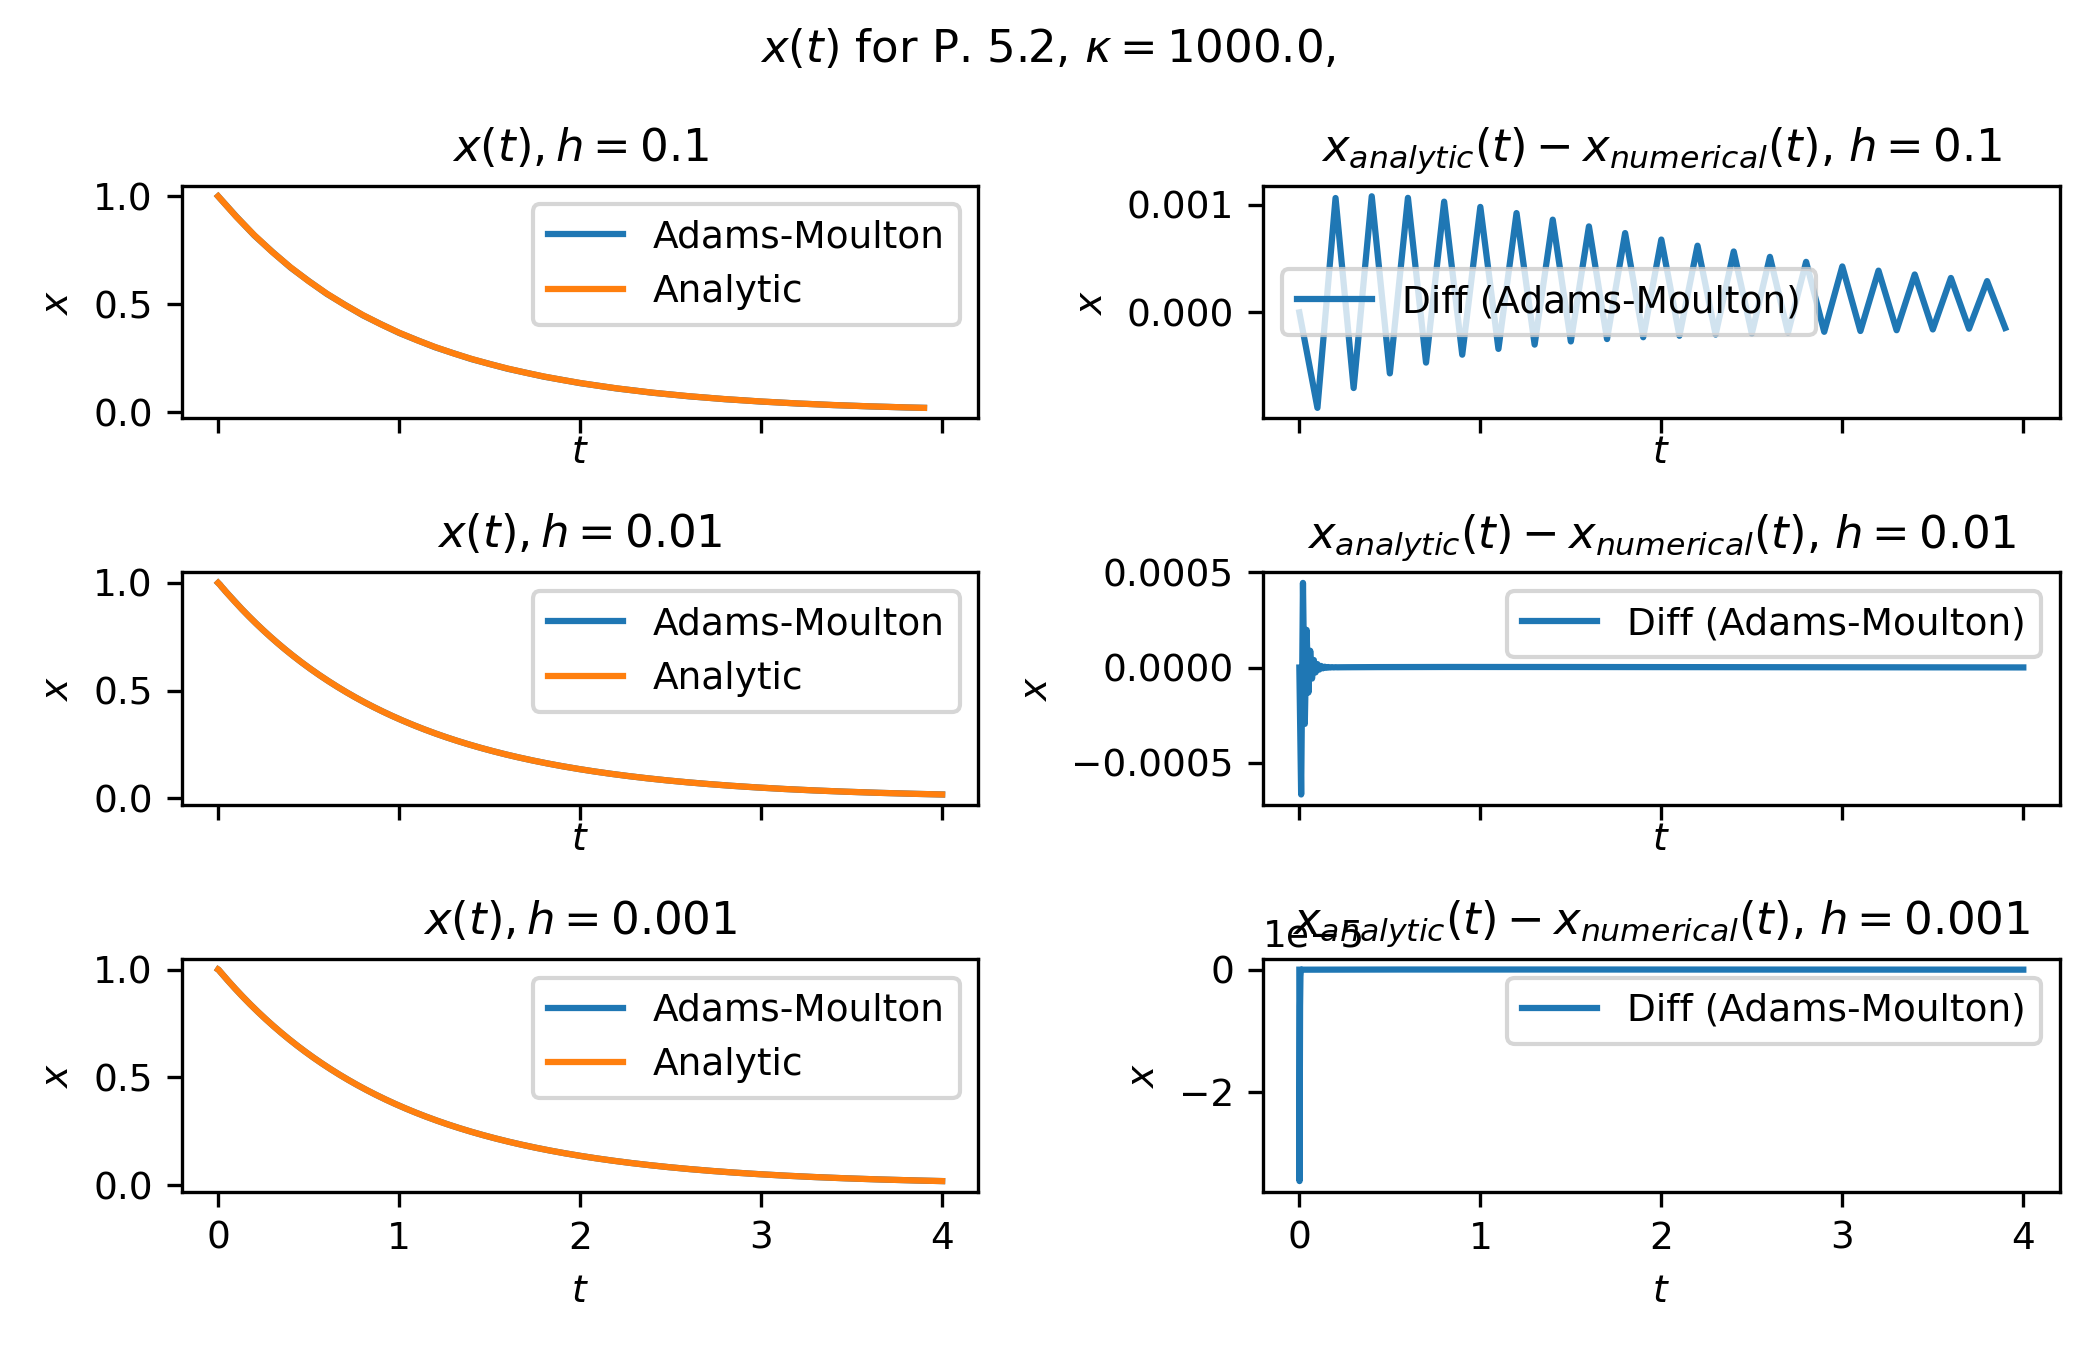
\includegraphics[width=0.9\textwidth]{../figures/p52.png}
        \caption{Problem 5.2. This plot shows an error analysis for the Adams-Moulton solver. We see that it is stable, despite the large step size and stiff problem in Case 2. We can compare these results with \cref{fig:problem32} to see the stability difference between the explicit Euler method and the implicit Adams-Moulton method.}
        \label{fig:problem52}
    \end{figure}
    \begin{figure}[h]
        \centering
        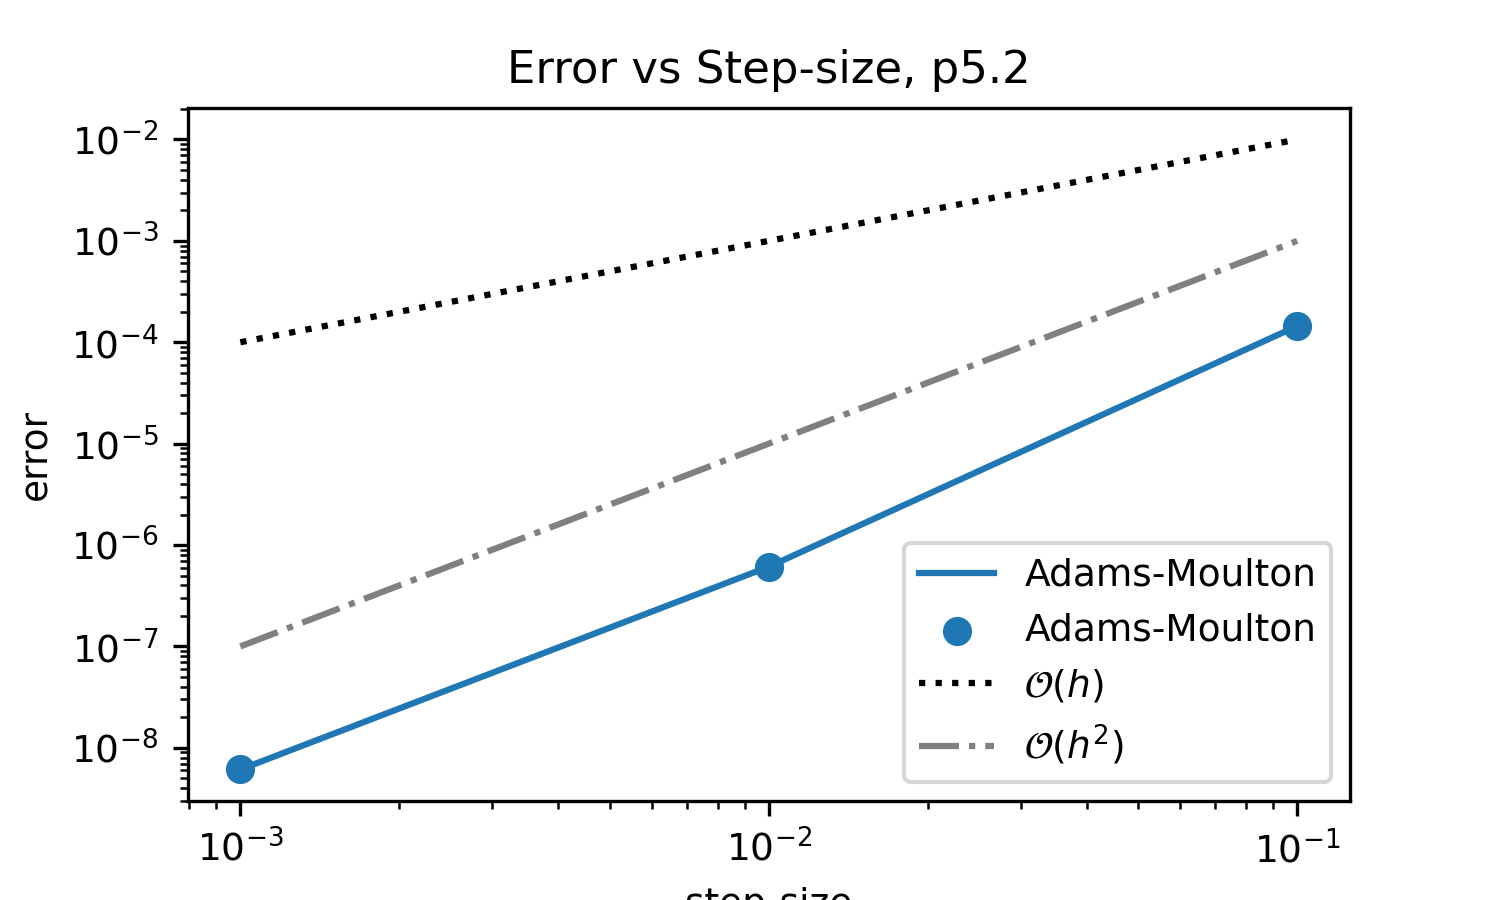
\includegraphics[width=0.9\textwidth]{../figures/p52err.png}
        \caption{Problem 5.2 error analysis. We see that the Adams-Moulton solver is 2nd order accurate, even at the large step size of $h = 0.1 \geq 0.002$. This solver is stable. A critical downside of using an implicit method is that it requires more computation time than the comparatively quick explicit methods; the solution to a set of linear equations must be calculated every step, which is expensive. However, because implicit solvers are stable at large step sizes, it may be faster to use an implicit method for stiff problems rather than an explicit method, which will require a very small step size for such problems.}
        \label{fig:problem52err}
    \end{figure}

\end{document}